% The tower of embeddings in the proof of the n-embeddings theorem:
% adjoin α₁, α₂, … one at a time, choosing at each stage an extension
% τᵢ of the previous embedding into ℂ.
% Source: book/tex/alg-NT/galois.tex (§ Embeddings into algebraic
% closures for number fields) — tikzcd.
\documentclass[border=2mm]{standalone}
\usepackage{tikz}
\usepackage{amssymb}
\usetikzlibrary{arrows.meta}
\begin{document}
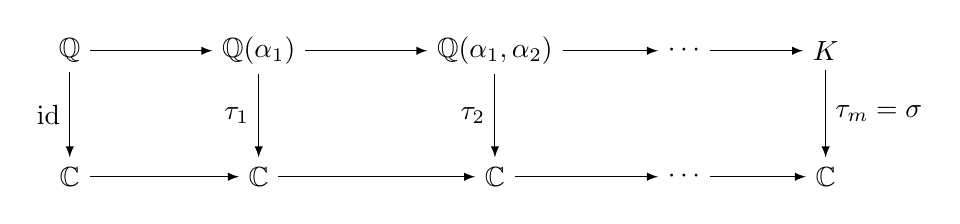
\begin{tikzpicture}[>=latex, row 1/.style={nodes={minimum width=1.6cm}}]
  \node (Q)  at (0,1.6)   {$\mathbb{Q}$};
  \node (Q1) at (2.4,1.6) {$\mathbb{Q}(\alpha_1)$};
  \node (Q2) at (5.4,1.6) {$\mathbb{Q}(\alpha_1,\alpha_2)$};
  \node (dots) at (7.8,1.6) {$\cdots$};
  \node (K)  at (9.6,1.6) {$K$};
  \node (C1) at (0,0)   {$\mathbb{C}$};
  \node (C2) at (2.4,0) {$\mathbb{C}$};
  \node (C3) at (5.4,0) {$\mathbb{C}$};
  \node (cdots) at (7.8,0) {$\cdots$};
  \node (C4) at (9.6,0) {$\mathbb{C}$};
  \draw[->] (Q) -- (Q1);
  \draw[->] (Q1) -- (Q2);
  \draw[->] (Q2) -- (dots);
  \draw[->] (dots) -- (K);
  \draw[->] (C1) -- (C2);
  \draw[->] (C2) -- (C3);
  \draw[->] (C3) -- (cdots);
  \draw[->] (cdots) -- (C4);
  \draw[->] (Q) -- (C1) node[midway,left] {$\mathrm{id}$};
  \draw[->] (Q1) -- (C2) node[midway,left] {$\tau_1$};
  \draw[->] (Q2) -- (C3) node[midway,left] {$\tau_2$};
  \draw[->] (K) -- (C4) node[midway,right] {$\tau_m=\sigma$};
\end{tikzpicture}
\end{document}
